\documentclass[]{article}
\usepackage{lmodern}
\usepackage{amssymb,amsmath}
\usepackage{ifxetex,ifluatex}
\usepackage{fixltx2e} % provides \textsubscript
\ifnum 0\ifxetex 1\fi\ifluatex 1\fi=0 % if pdftex
  \usepackage[T1]{fontenc}
  \usepackage[utf8]{inputenc}
\else % if luatex or xelatex
  \ifxetex
    \usepackage{mathspec}
  \else
    \usepackage{fontspec}
  \fi
  \defaultfontfeatures{Ligatures=TeX,Scale=MatchLowercase}
\fi
% use upquote if available, for straight quotes in verbatim environments
\IfFileExists{upquote.sty}{\usepackage{upquote}}{}
% use microtype if available
\IfFileExists{microtype.sty}{%
\usepackage{microtype}
\UseMicrotypeSet[protrusion]{basicmath} % disable protrusion for tt fonts
}{}
\usepackage[margin=1in]{geometry}
\usepackage{hyperref}
\hypersetup{unicode=true,
            pdftitle={Relatório IC},
            pdfauthor={Fernanda Buzza Alves Barros},
            pdfborder={0 0 0},
            breaklinks=true}
\urlstyle{same}  % don't use monospace font for urls
\usepackage{graphicx,grffile}
\makeatletter
\def\maxwidth{\ifdim\Gin@nat@width>\linewidth\linewidth\else\Gin@nat@width\fi}
\def\maxheight{\ifdim\Gin@nat@height>\textheight\textheight\else\Gin@nat@height\fi}
\makeatother
% Scale images if necessary, so that they will not overflow the page
% margins by default, and it is still possible to overwrite the defaults
% using explicit options in \includegraphics[width, height, ...]{}
\setkeys{Gin}{width=\maxwidth,height=\maxheight,keepaspectratio}
\IfFileExists{parskip.sty}{%
\usepackage{parskip}
}{% else
\setlength{\parindent}{0pt}
\setlength{\parskip}{6pt plus 2pt minus 1pt}
}
\setlength{\emergencystretch}{3em}  % prevent overfull lines
\providecommand{\tightlist}{%
  \setlength{\itemsep}{0pt}\setlength{\parskip}{0pt}}
\setcounter{secnumdepth}{0}
% Redefines (sub)paragraphs to behave more like sections
\ifx\paragraph\undefined\else
\let\oldparagraph\paragraph
\renewcommand{\paragraph}[1]{\oldparagraph{#1}\mbox{}}
\fi
\ifx\subparagraph\undefined\else
\let\oldsubparagraph\subparagraph
\renewcommand{\subparagraph}[1]{\oldsubparagraph{#1}\mbox{}}
\fi

%%% Use protect on footnotes to avoid problems with footnotes in titles
\let\rmarkdownfootnote\footnote%
\def\footnote{\protect\rmarkdownfootnote}

%%% Change title format to be more compact
\usepackage{titling}

% Create subtitle command for use in maketitle
\newcommand{\subtitle}[1]{
  \posttitle{
    \begin{center}\large#1\end{center}
    }
}

\setlength{\droptitle}{-2em}

  \title{Relatório IC}
    \pretitle{\vspace{\droptitle}\centering\huge}
  \posttitle{\par}
    \author{Fernanda Buzza Alves Barros}
    \preauthor{\centering\large\emph}
  \postauthor{\par}
      \predate{\centering\large\emph}
  \postdate{\par}
    \date{\_\_ de \_\_\_\_\_\_\_\_ de \_\_\_\_}


\begin{document}
\maketitle

\section{INTRODUÇÃO}\label{introducao}

Problemas de dados faltantes em pesquisa são recorrentes em bancos de
dados. Para a solução desses problemas existem vários métodos que podem
ser utilizados. Entretanto, todos os métodos possuem uma questão
principal: como inferir os valores não observados?

Para a resposta dessa pergunta, temos que o ideal seria ter os dados,
porém na falta deles temos que utilizar o método que melhor se ajusta a
distribuição dos dados.

Nessa pesquisa utilizaremos o método proposto por Rubin (1987), Van
Buuren e Groothuis-Oudshoorn (2011), que é conhecido como Imputação
Múltipla.

\section{METODOLOGIA}\label{metodologia}

A Imputação Múltipla consiste em gerar valores (m vezes) para os dados
faltantes, ela cria uma matriz com todas as M imputações. Para gerar
essas imputações existem alguns métodos, como por exemplo
\emph{Predictive Mean Matching (pmm)} e \emph{Unconditional Mean
Imputation (mean)}, que serão os métodos utilizados nesse estudo.

\subsection{Predictive Mean Matching
(pmm)}\label{predictive-mean-matching-pmm}

\subsection{Unconditional Mean Imputation
(mean)}\label{unconditional-mean-imputation-mean}

\section{RESULTADOS}\label{resultados}

\subsection{Banco de dados}\label{banco-de-dados}

Para realizar a imputação dos dados utilizamos o banco de dados \emph{US
Term Life insurance} do pacote \emph{CASdatasets} disponível no software
R. As imputações e os resultados foram obtidos utilizando esse mesmo
software estatístico. O banco de dados possui 18 variáveis com 500
observações, como pode ser visto abaixo.

\begin{verbatim}
## 'data.frame':    500 obs. of  18 variables:
##  $ Gender         : int  1 1 1 1 1 1 0 1 1 1 ...
##  $ Age            : int  30 50 39 43 61 34 75 29 35 70 ...
##  $ MarStat        : int  1 1 1 1 1 2 0 1 2 1 ...
##  $ Education      : int  16 9 16 17 15 11 8 16 4 17 ...
##  $ Ethnicity      : int  3 3 1 1 1 2 1 1 3 1 ...
##  $ SmarStat       : int  2 1 2 1 2 1 0 2 1 2 ...
##  $ Sgender        : int  2 2 2 2 2 2 0 2 2 2 ...
##  $ Sage           : int  27 47 38 35 59 31 0 31 45 74 ...
##  $ Seducation     : int  16 8 16 14 12 14 0 17 9 16 ...
##  $ NumHH          : int  3 3 5 4 2 4 1 3 2 2 ...
##  $ Income         : int  43000 12000 120000 40000 25000 28000 2500 100000 20000 101000 ...
##  $ TotIncome      : int  43000 0 90000 40000 1020000 0 0 84000 0 6510000 ...
##  $ Charity        : int  0 0 500 0 500 0 0 0 0 284000 ...
##  $ Face           : int  20000 130000 1500000 50000 0 220000 0 600000 0 0 ...
##  $ FaceCVLifePol  : int  0 0 0 75000 7000000 0 14000 0 0 2350000 ...
##  $ CashCVLifePol  : int  0 0 0 0 300000 0 5000 0 0 0 ...
##  $ BorrowCVLifePol: int  0 0 0 5 5 0 5 0 0 5 ...
##  $ NetValue       : int  0 0 0 0 0 0 0 0 0 0 ...
\end{verbatim}

Porém selecionamos as seguintes variáveis para realizar a pesquisa:
Gênero (gênero do entrevistado); Idade (idade do entrevistado); Estado
Civil (estado civil do entrevistado); Escolaridade (número de anos de
escolaridade do entrevistado); Etnia (etnia do entrevistado); Renda
(renda anual da família do entrevistado).

Primeiras observações do banco de dados original:

\begin{verbatim}
##   Gender Age MarStat Education Ethnicity Income
## 1      1  30       1        16         3  43000
## 2      1  50       1         9         3  12000
## 3      1  39       1        16         1 120000
## 4      1  43       1        17         1  40000
## 5      1  61       1        15         1  25000
## 6      1  34       2        11         2  28000
\end{verbatim}

\subsection{Análise Descritiva}\label{analise-descritiva}

Após a escolha das variáveis para esse estudo, iremos realizar uma
análise descritiva de cada uma delas, e assim avaliar as relações
existentes entre a variável resposta e as covariáveis do banco de dados.
Ao final realizaremos um dos principais objetivos dessa pesquisa, que é
verificar os possíveis questionamentos sobre a Renda a partir das outras
variáveis.

Primeiramente analisaremos as variáveis individualmente, com interesse
em suas distribuições e comportamentos. Pelos dados observamos que as
variáveis contínuas são: Renda, Idade e Escolaridade, e as variáveis
discretas são: Gênero, Estado Civil e Etnia.

\begin{flushleft}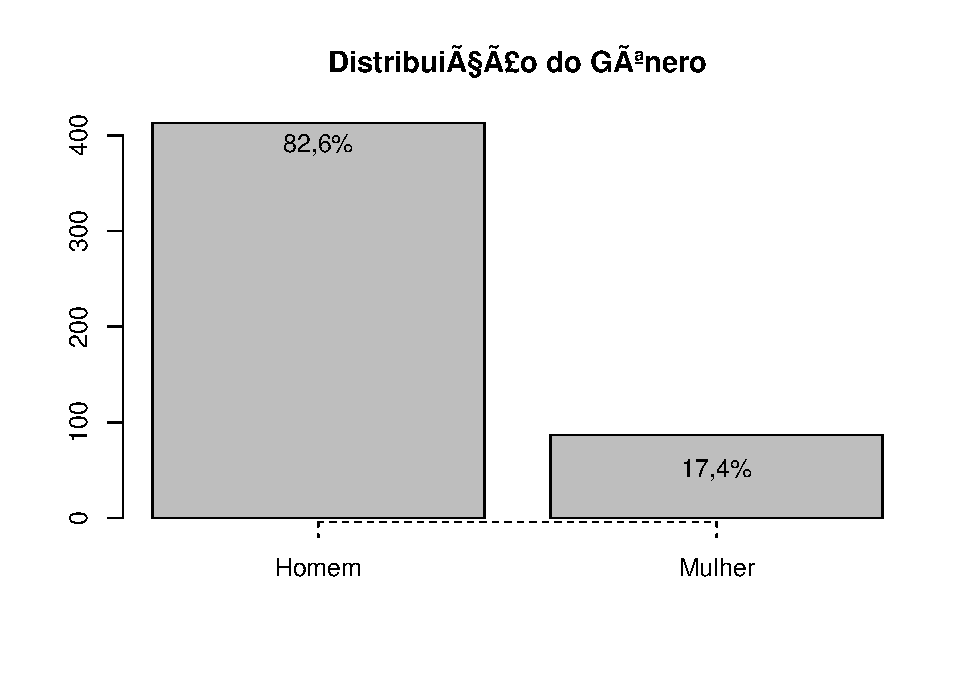
\includegraphics{Relatorio_IC_files/figure-latex/unnamed-chunk-6-1} \end{flushleft}

Para as variáveis discretas temos que o banco de dados possui uma
quantidade maior de entrevistados do sexo masculino do que do sexo
feminino; para o estado civil temos uma concentração maior de respostas
para os entrevistados casados e uma menor quantidade de entrevistados
com o estado civil de morando juntos; por fim para a etnia temos uma
maior quantidade de entrevistados que possuem etnia Branco, sendo que as
outras etnias possuem valores menores de entrevistados no banco de
dados.

\begin{flushleft}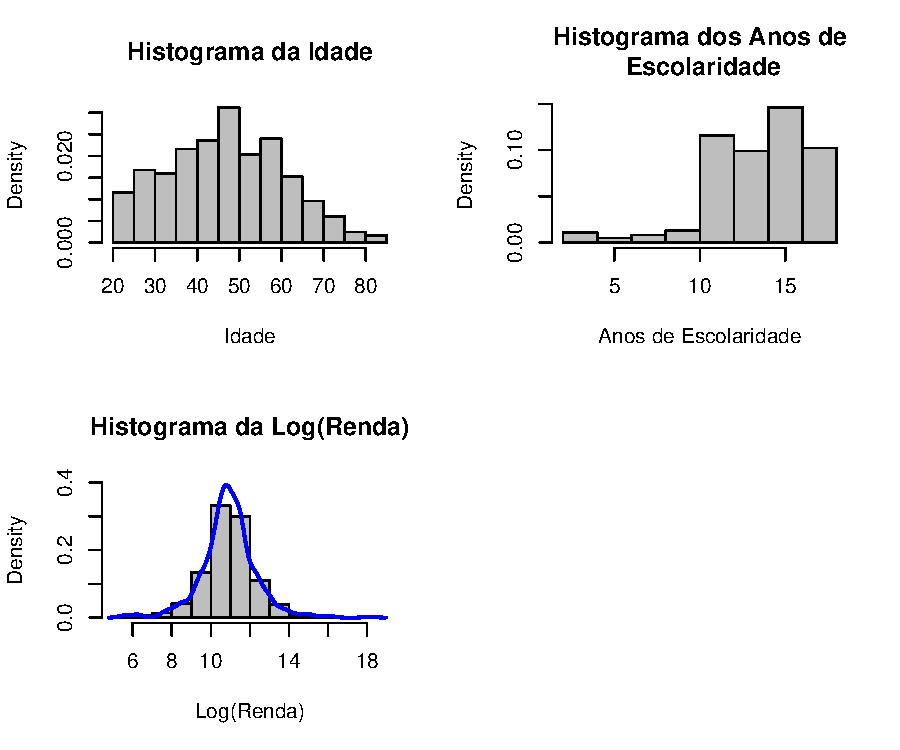
\includegraphics{Relatorio_IC_files/figure-latex/unnamed-chunk-7-1} \end{flushleft}

Para as variáveis contínuas temos que a variável Idade está bastante
distribuída entre os 20 anos e 70 anos, após 70 anos vemos poucos
entrevistados no banco de dados, sendo também que a idade máxima é 85
anos e a idade mínima é 20 anos. A média é 47.164 anos e a mediana 47
anos. O primeiro quantil é de 37 anos, representando a idade que deixa
25\% das observações abaixo e 75\% acima dessa idade. E o terceiro
quantil é de 58 anos, representando a idade que possui 75\% das
observações abaixo dela e 25\% das observações acima dela.

A distribuição da variável Escolaridade possui maior concentração de
entrevistados após 10 anos de escolaridade.

E para a variável Renda temos que a renda mínima anual é 260 dólares e a
renda máxima anual é 75000000 dólares. A mediana e a média são
5.4\times 10\^{}\{4\} dólares e 3.210219\times 10\^{}\{5\} doláres,
respectivamente. O primeiro quantil é de 2.8\times 10\^{}\{4\} dólares,
representando o valor de renda anual que deixa 25\% das observações
abaixo dela e 75\% acima deela. E o terceiro quantil é de
1.06\times 10\^{}\{5\} dólares, representando a renda anual que possui
75\% das observações abaixo dela e 25\% das observações acima dela.
Aplicamos o logarítimo para melhor visualização da distribuição da renda
anual através do histograma e percebemos uma aparência com a
distribuição normal.

Além da análise da variável Escolaridade em anos, foi realizada também a
análise dos anos de escolaridade divididos pelos tipos de ensino
existentes, que são: 2-10 anos de escolaridade é o Ensino Fundamental,
11-14 anos de escolaridade é o Ensino Médio e de 15-17 anos de
escolaridade é o Ensino Superior, assim obtemos:

\begin{flushleft}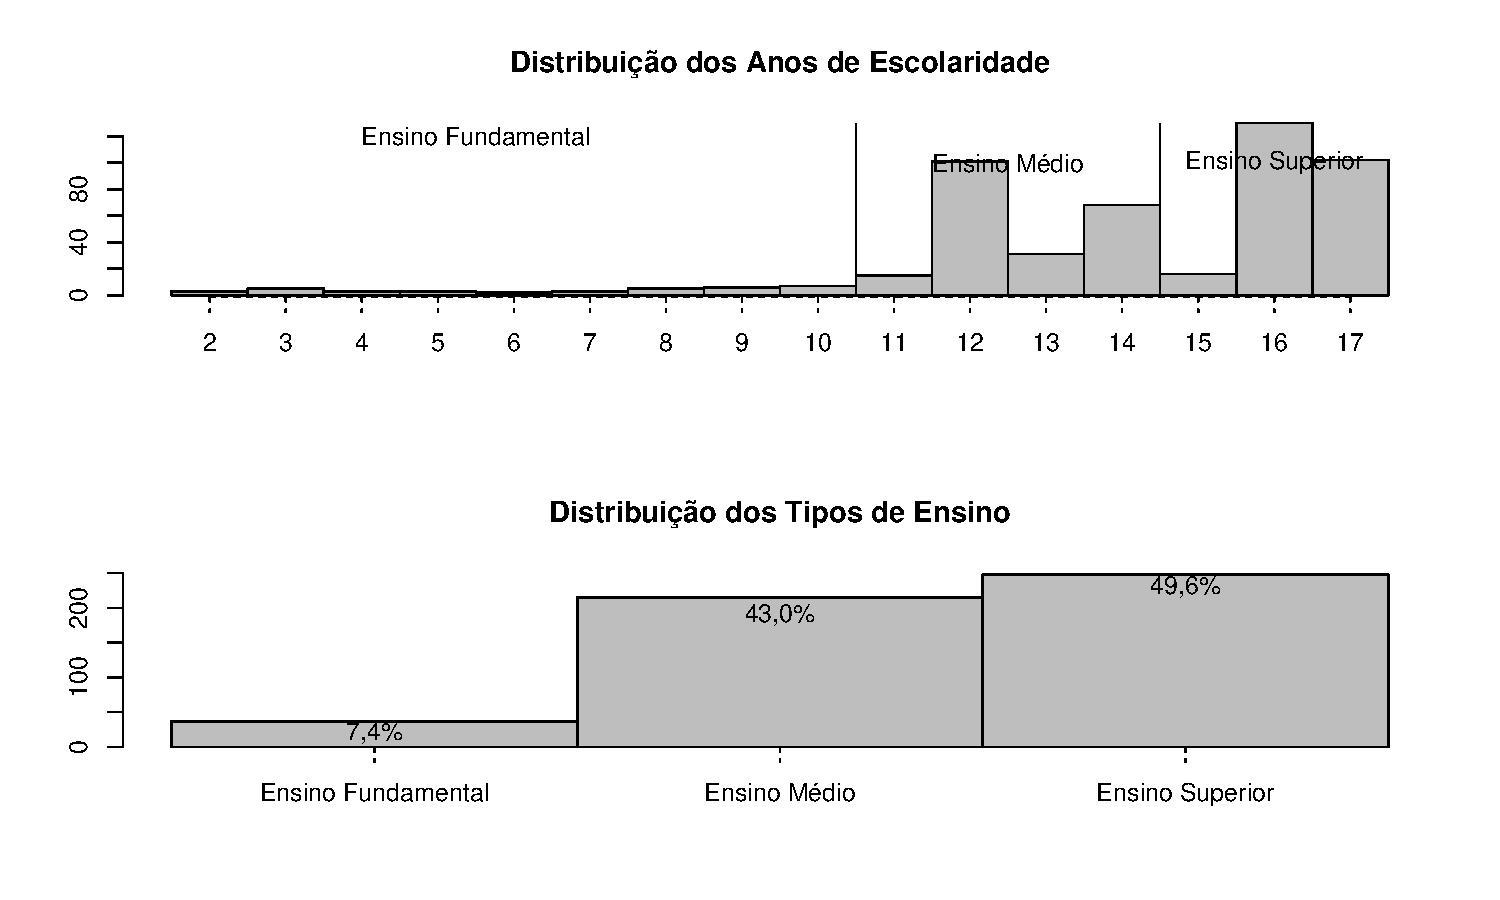
\includegraphics{Relatorio_IC_files/figure-latex/unnamed-chunk-8-1} \end{flushleft}

Avaliando os tipos de ensino percebemos uma maior concentração de
entrevistados que possuem o ensino médio e o ensino superior, sendo que
quase a metade dos entrevistados possuem ensino superior, esse valor
corresponde a 248 entrevistados.

Analisamos também a relação entre a variável resposta (Renda) e as
covariáveis presentes no banco de dados escolhido. Assim obtivemos os
seguintes resultados:

\begin{flushleft}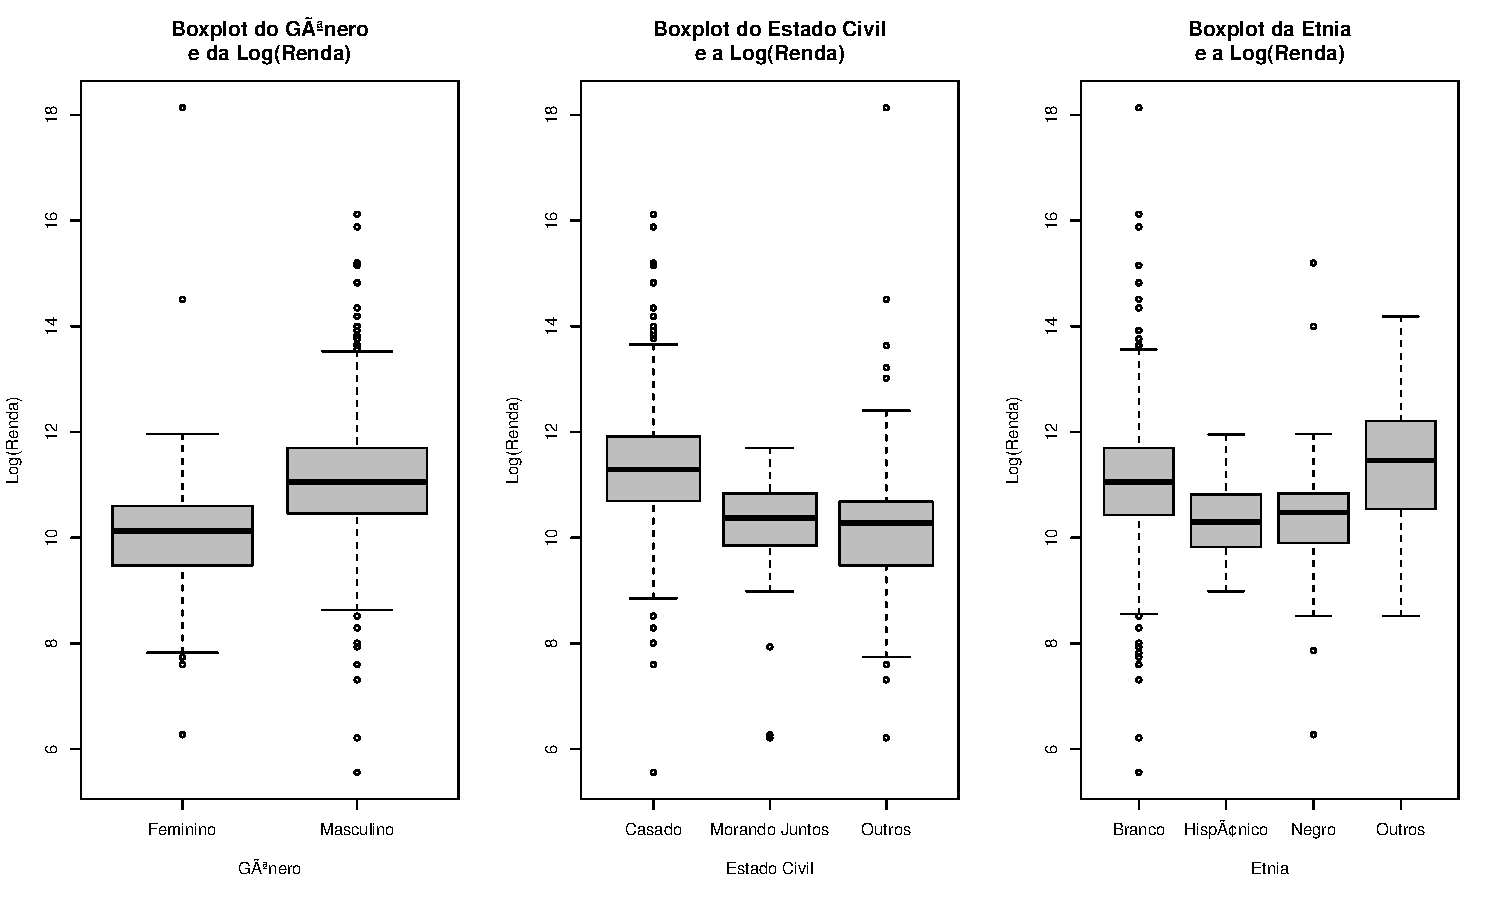
\includegraphics{Relatorio_IC_files/figure-latex/unnamed-chunk-9-1} \end{flushleft}

Para as variáveis discretas temos os boxplots da Log(Renda) com cada uma
das variáveis separadamente. Para o gênero observamos um valor de renda
maior para o sexo masculino, comparando com o sexo feminino; já a
variável Estado Civil os entrevistados casados possuem uma renda maior,
seguido pelos que moram juntos com o parceiro(a) e depois os que estão
na categoria de outro tipo de estado civil. Na comparação entre a
Log(Renda) e a Etnia percebemos uma renda maior para a categoria outros
da etnia, entretanto, como foi observado anteriormente, esta categoria
representa somente 5\% do total do banco de dados.

\begin{flushleft}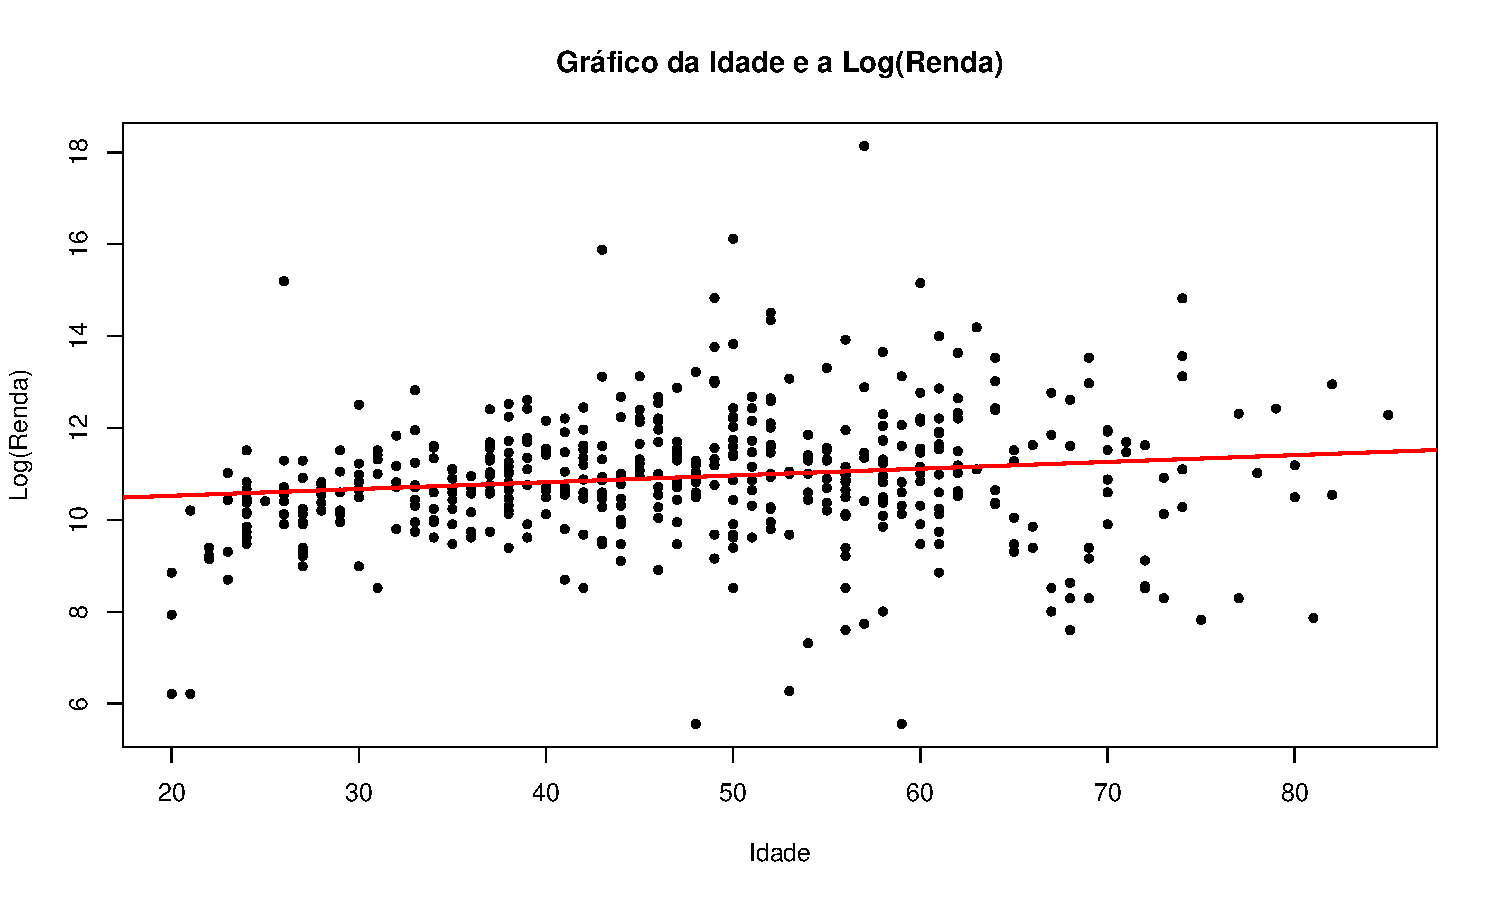
\includegraphics{Relatorio_IC_files/figure-latex/unnamed-chunk-10-1} \end{flushleft}

Para a relação entre as variáveis Log(Renda) e a Idade temos o gráfico
de dispersão acima, nele percebemos uma pequena inclinação no ajuste da
curva quando ocorre o aumento das idades dos entrevistados, o que indica
um possível ganho de renda anual maior para os entrevistados a medida
que aumenta a idade.

\begin{flushleft}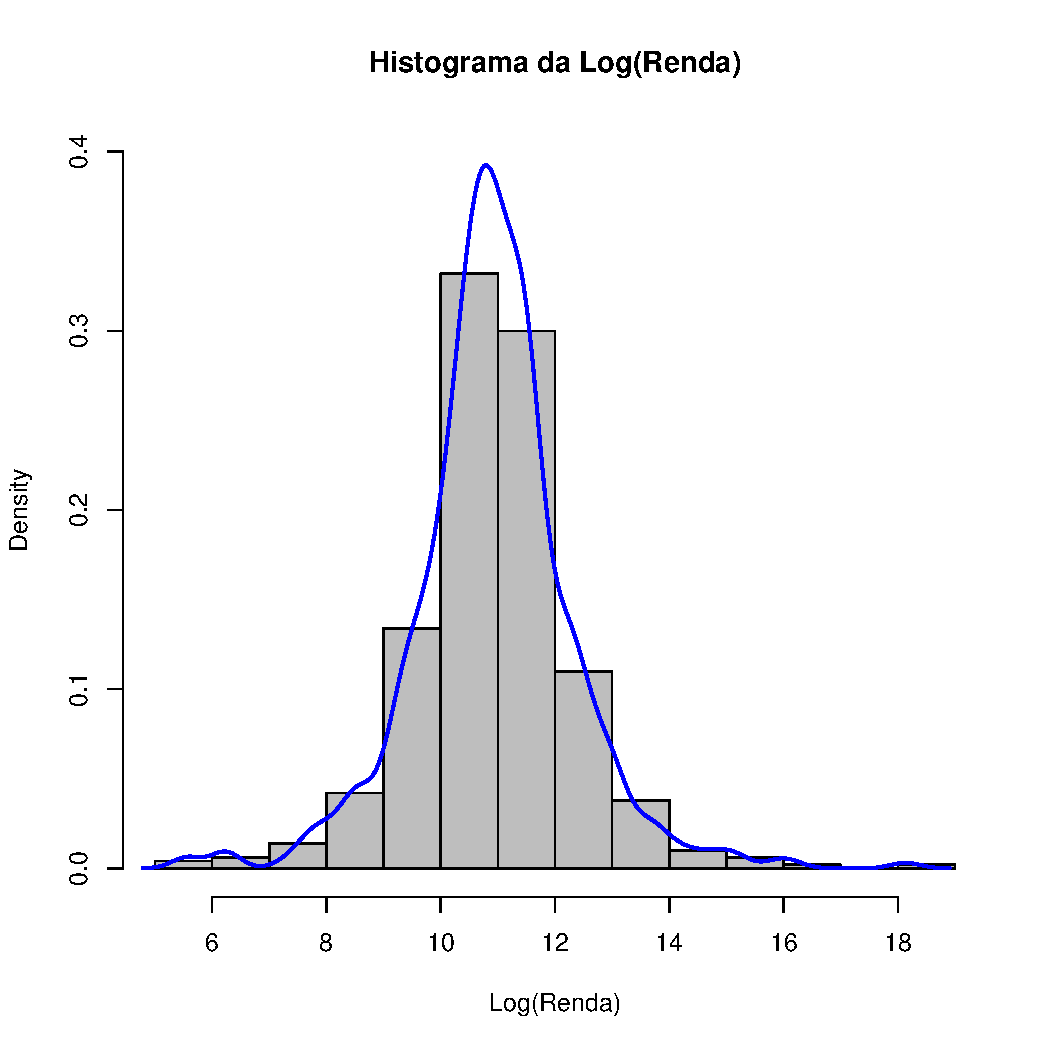
\includegraphics{Relatorio_IC_files/figure-latex/unnamed-chunk-11-1} \end{flushleft}

Avaliando a relação entre as variáveis Log(Renda) e a recodificação da
variável Anos de Escolaridade, variável separada em tipos de ensino para
melhor visualização da relação existente, temos que o tipo de ensino
influencia na renda dos entrevistados. Assim observamos valores de renda
maiores para o Ensino Superior, que possui de 15-17 anos de
escolaridade.

Analisaremos as relações entre as variáveis selecionadas do banco de
dados original. Temos interesse em responder as seguintes perguntas:

\begin{itemize}
\item
  Como está distribuída a variável Renda.
\item
  Qual é a relação entre a Renda e o Gênero.
\item
  Com maiores anos de escolaridade há aumento da renda.
\item
  O estado civil tem influência na renda.
\item
  Avaliar a relação entre a etnia e a renda.
\end{itemize}

O mínimo de anos de escolaridade é 2 anos e o máximo é 17 anos. A
mediana e a média são 14 anos e 14,06 anos, respectivamente. E o
primeiro quantil é 12 anos e o terceiro quantil é 16 anos.

Essa variável possui como renda mínima 260 dólares e renda máxima
75.000.000 dólares. A mediana e a média são 54.000 dólares e 321.022
doláres, respectivamente. E o primeiro e terceiro quantis são 28.000
dólares e 106.000 dólares.

Por fim, avaliando as variáveis Estado Civil, Gênero e Etnia temos:

Sendo assim a pesquisa possui 87 respondentes do sexo feminino e 413
respondentes do sexo masculino.

\subsubsection{Distribuição da Renda}\label{distribuicao-da-renda}

Pelo histograma podemos avaliar a distribuição da variável Renda, a
partir dos dados retirados do banco de dados original. Observamos uma
maior concentração de valores entre o Log(Renda) de 10 a 12. Nas caldas
podemos perceber reduções de valores da renda familiar.

\subsubsection{Renda e Gênero}\label{renda-e-genero}

Ao plotarmos os boxplots da Log(Renda) e o Gênero vemos a relação entre
os valores da renda dos homens comparados com os das mulheres. Nesse
caso os homens possuem maiores valores de renda do que as mulheres.

\subsubsection{Renda e Anos de
Escolaridade}\label{renda-e-anos-de-escolaridade}

Ao analisar o efeito na quantidade de Anos de Escolaridade e a Renda,
percebemos um crescimento na quantidade ganha de renda de acordo com os
anos de escolaridade. Observamos que com a inclusão da reta pontilhada
em vermelho, que representa a média da variável Log(Renda), a
possibilidade de determinar os anos de escolaridade que estão acima da
média de valores ganhos de renda. Entre os anos de escolaridade de 2 a 8
anos não percebemos uma relação crescente, sendo que há uma queda em 4,
5 e 8 anos de escolaridade, que pode ser devido a quantidade de
entrevistados desses grupos representados no banco de dados; o que pode
ser verificado na tabela abaixo:

\subsubsection{Renda e Estado Civil}\label{renda-e-estado-civil}

Para analisar a relação entre o Estado Civil e a Log(Renda) percebemos
que as pessoas casadas possuem uma renda maior, quando comparado com os
outros grupos apresentados pelo banco de dados.

\subsubsection{Renda e Etnia}\label{renda-e-etnia}

Para avaliar a relação entre a Etnia e a Log(Renda) observamos maiores
valores de renda para o grupo white e o others, sendo que os grupos
black e hispanic apresentam similaridades nos valores de renda.

\subsubsection{Renda, Idade e Gênero}\label{renda-idade-e-genero}

\subsection{Imputação}\label{imputacao}

O banco de dados não possui dados faltantes, portanto para avaliar a
Renda (variável de interesse) foi necessário gerar os dados faltantes.
Sendo assim utilizamos uma distribuição binomial com probabilidade de
sucesso de 0.2 para a criar dos dados faltantes na variável Renda, e
utilizamos a função de fixa a semente ao gerar os números aleatórios.

Primeiras observações do banco de dados com dados faltantes na variável
Renda:

\begin{verbatim}
##   Gender Age MarStat Education Ethnicity Income
## 1      1  30       1        16         3     NA
## 2      1  50       1         9         3  12000
## 3      1  39       1        16         1 120000
## 4      1  43       1        17         1  40000
## 5      1  61       1        15         1     NA
## 6      1  34       2        11         2  28000
\end{verbatim}

Assim para realizar a imputação utilizamos o pacote \emph{Multivariate
Imputation With Chained Equations (MICE)}. A função que realiza a
imputação chama-se mice, e nesse estudo realizamos a imputação 5 vezes
(m=5) tanto para o método da \emph{PMM} e da \emph{Mean} da função para
comparar os resultados.

Abaixo temos o output da função de imputação com as principais
informações.

\section{CONCLUSÃO}\label{conclusao}

\section{REFERÊNCIAS BIBLIOGRÁFICAS}\label{referencias-bibliograficas}

Rubin (1987)

Van Buuren, S., Groothuis-Oudshoorn, K. (2011). mice: Multivariate
Imputation by Chained Equations in R. Journal of Statistical Software,
45(3), 1-67. \href{http://www.jstatsoft.org/v45/i03/}{linked phrase}

Morris TP, White IR, Royston P (2015). Tuning multiple imputation by
predictive mean matching and local residual draws. BMC Med Res Methodol.
;14:75.

Frees, E.W. (2011). Regression Modeling with Actuarial and Financial
Applications, Cambridge University Press.


\end{document}
